\documentclass[12pt]{article}

\usepackage[margin=1in]{geometry}

\usepackage{amsmath,amssymb,wasysym}
\usepackage{graphicx}
\usepackage[subrefformat=parens,labelformat=parens]{subcaption}

\usepackage{cleveref}

\title{NNM Results for 2-DOF Nonlinear System}
\date{2023/02/06}
\begin{document}
\maketitle{}

\tableofcontents{}

The general form of the nonlinear system considered is,
\begin{align}
  \begin{bmatrix} 1 & 0\\ 0 & 1 \end{bmatrix}
  \begin{Bmatrix} \ddot{x}_1\\ \ddot{x}_2 \end{Bmatrix} +
  \beta \begin{bmatrix} 0 & 0\\ 0 & 1 \end{bmatrix}
  \begin{Bmatrix} \dot{x}_1\\ \dot{x}_2 \end{Bmatrix} &+
  \begin{bmatrix} 2 & -1\\ -1 & 2 \end{bmatrix}
  \begin{Bmatrix} \ddot{x}_1\\ \ddot{x}_2 \end{Bmatrix} +
  \begin{Bmatrix}
    \alpha x_1^3\\ \gamma \dot{x}_2^3 + f_{fr}(\dot{x}_2)
  \end{Bmatrix} =
  \begin{Bmatrix}
    F \cos\Omega t\\ 0
  \end{Bmatrix}, \label{eq:nleqgform}\\
  \text{with, } f_{fr}(\dot{x}_2) & \begin{cases} \in (-\mu N, \mu N)
                                      & \dot{x}_2=0\\ \mu N
                                      =sgn(\dot{x}_2) &
                                                       otherwise \end{cases}. 
\end{align}
The friction model $f_{fr}(\cdot)$ is a \textbf{set-valued Coulomb
  law} that is implemented using a \textbf{Dynamic Lagrangian
  Framework}.

For all the results that follow, the damping parameter $\beta=0.1 N s
m^{-1}$ and $\gamma=0$. 

\pagebreak
\section{Comparisons with Transient Simulations}
\label{sec:comp-with-trans}

\textbf{Note}: Transients calculated using an average acceleration
implicit Newmark-$\beta$ implementation.

\begin{figure}[!h]
  \centering
  \begin{subfigure}{0.5\textwidth}
    \centering
    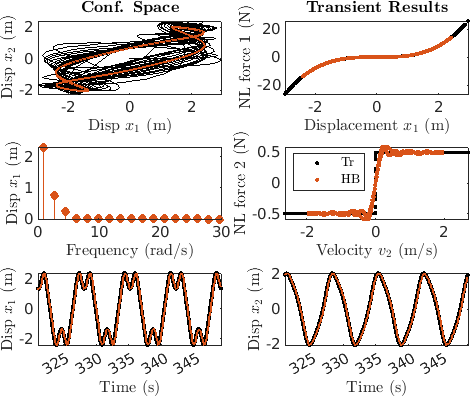
\includegraphics[width=\linewidth]{FIGS/A_TrComp_33}
    \caption{}
  \end{subfigure}%
  \begin{subfigure}{0.5\textwidth}
    \centering
    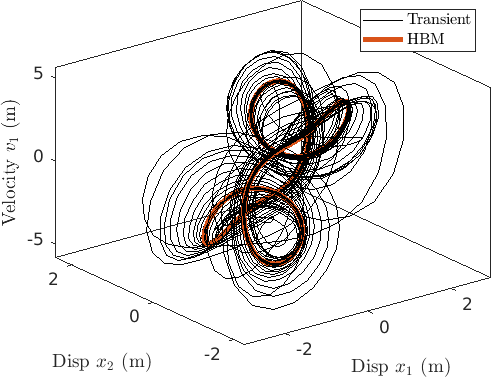
\includegraphics[width=\linewidth]{FIGS/A_TrCompSS_33}
    \caption{}
  \end{subfigure}
  \caption{Comparisons between transient simulations and Harmonic
    Balance for Forced Response}
\end{figure}

\begin{table}[!h]
  \centering
  \caption{Parameters Used}
  \begin{tabular}[t]{c|c}
    \hline\hline
    \textbf{Parameter} & \textbf{Value}\\\hline
    $\beta$ & $0.1\,Ns m^{-1}$\\
    $\alpha$ & $1\, N m^{-1}$\\
    $\gamma$ & $0\, Ns^3 m^{-3}$\\
    $\mu N$ & $0.5\, N$\\
    $\Omega$ & $0.9\, rad/s$\\
    $F$ & $10\, N$\\
    \hline\hline
  \end{tabular}
\end{table}

\pagebreak
\section{Forced Response Results}
\label{sec:forc-resp-results}

\begin{figure}[!h]
  \centering
  \begin{subfigure}{0.5\textwidth}
    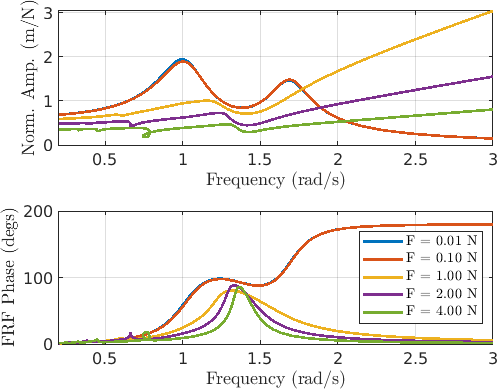
\includegraphics[width=\linewidth]{FIGS/B_FRESP_hi1_33}
    \caption{First Harmonic}
  \end{subfigure}%
  \begin{subfigure}{0.5\textwidth}
    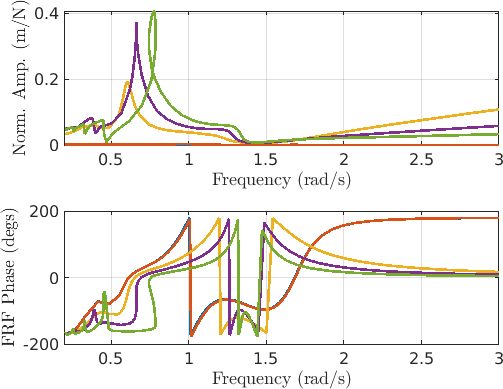
\includegraphics[width=\linewidth]{FIGS/B_FRESP_hi3_33}
    \caption{Third Harmonic}
  \end{subfigure}

  \begin{subfigure}{0.5\textwidth}
    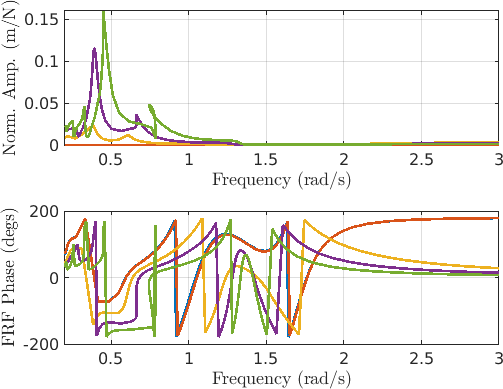
\includegraphics[width=\linewidth]{FIGS/B_FRESP_hi5_33}
    \caption{Fifth Harmonic}
  \end{subfigure}%
  \begin{subfigure}{0.5\textwidth}
    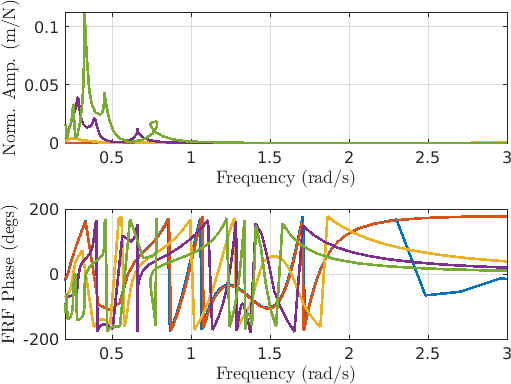
\includegraphics[width=\linewidth]{FIGS/B_FRESP_hi7_33}
    \caption{Seventh Harmonic}
  \end{subfigure}  
  \caption{Different harmonic components of system response (plotted,
    $x_1$) to steady state forcing (a total of 33 harmonics were
    considered for the balance)}
\end{figure}


\begin{table}[!h]
  \centering
  \caption{Parameters Used}
  \begin{tabular}[t]{c|c}
    \hline\hline
    \textbf{Parameter} & \textbf{Value}\\\hline
    $\beta$ & $0.1\,Ns m^{-1}$\\
    $\alpha$ & $1\, N m^{-1}$\\
    $\gamma$ & $0\, Ns^3 m^{-3}$\\
    $\mu N$ & $0.5\, N$\\
    $\Omega$ & $[0.1,\, 3.0]\, rad/s$\\
    $F$ & $[0.01,\, 4.0]\, N$\\
    \hline\hline
  \end{tabular}
\end{table}

\pagebreak

\section{EPMC Results}
\label{sec:epmc-results}

\begin{figure}[!h]
  \centering
  \begin{subfigure}{0.5\textwidth}
    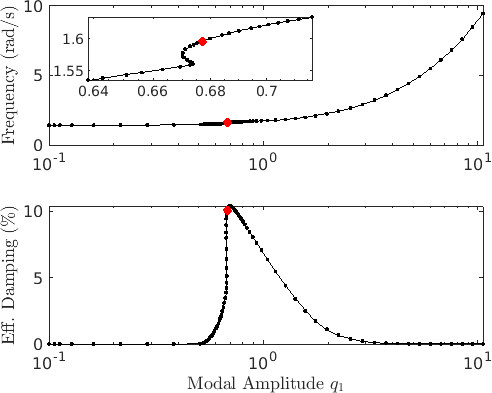
\includegraphics[width=\linewidth]{FIGS/C_EPMCBB_33}
    \caption{Backbone}
  \end{subfigure}%
  \begin{subfigure}{0.5\textwidth}
    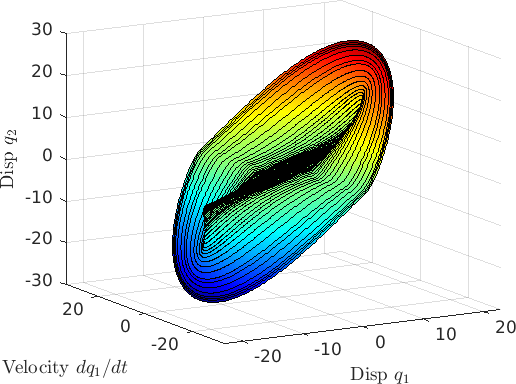
\includegraphics[width=\linewidth]{FIGS/C_EPMCIM_33}
    \caption{``Invariant'' Manifold}
  \end{subfigure}
  \caption{Backbone and ``invariant'' manifold computed using EPMC (33
  harmoincs considered for the balance). Manifold plotted until the
  red colored point in the backbone.}
\end{figure}

\begin{table}[!h]
  \centering
  \caption{Parameters Used}
  \begin{tabular}[t]{c|c}
    \hline\hline
    \textbf{Parameter} & \textbf{Value}\\\hline
    $\beta$ & $0.1\,Ns m^{-1}$\\
    $\alpha$ & $1\, N m^{-1}$\\
    $\gamma$ & $0\, Ns^3 m^{-3}$\\
    $\mu N$ & $0.5\, N$\\
    $\Omega$ & N/A\\
    $F$ & N/A\\
    \hline\hline
  \end{tabular}
\end{table}

\pagebreak
\section{Influence of Harmonic Truncation}
\label{sec:influence-hamronics}

\begin{figure}[!h]
  \centering
  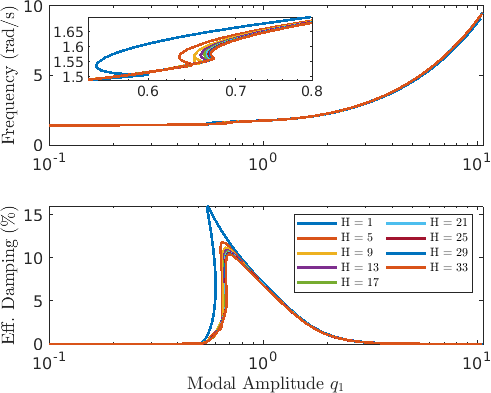
\includegraphics[width=0.6\linewidth]{FIGS/D_EPMCBBHCOMP}
  \caption{Influence of Harmonic Truncation on the Computed Backbones}
\end{figure}

\begin{table}[!h]
  \centering
  \caption{Parameters Used}
  \begin{tabular}[t]{c|c}
    \hline\hline
    \textbf{Parameter} & \textbf{Value}\\\hline
    $\beta$ & $0.1\,Ns m^{-1}$\\
    $\alpha$ & $1\, N m^{-1}$\\
    $\gamma$ & $0\, Ns^3 m^{-3}$\\
    $\mu N$ & $0.5\, N$\\
    $\Omega$ & N/A\\
    $F$ & N/A\\
    \hline\hline
  \end{tabular}
\end{table}

\pagebreak
\section{Influence of Parameters}
\label{sec:influence-parameters-1}

\begin{figure}[!h]
  \centering
  \begin{subfigure}{0.5\textwidth}
    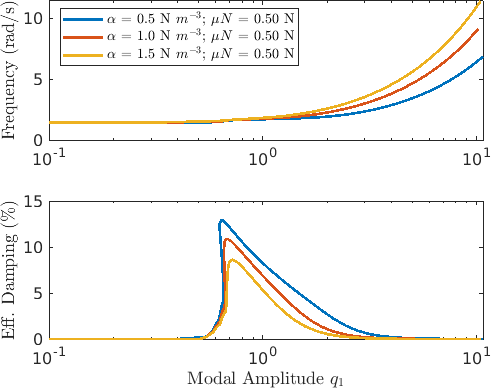
\includegraphics[width=\linewidth]{FIGS/E_EPMCBBPCOMP_13_alvar}
    \caption{}
  \end{subfigure}%
  \begin{subfigure}{0.5\textwidth}
    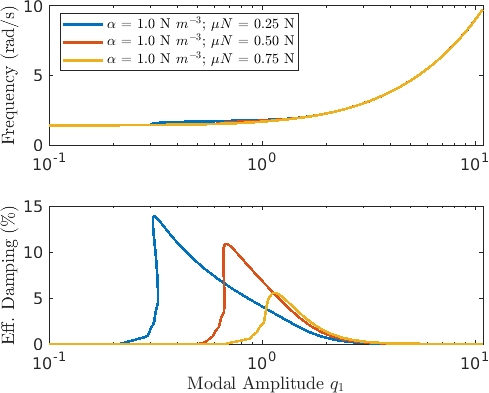
\includegraphics[width=\linewidth]{FIGS/E_EPMCBBPCOMP_13_muvar}
    \caption{}
  \end{subfigure}  
  \caption{Influence of (a) $\alpha$ and (b) $\mu N$ on the backbones
    when the other is kept constant (13 harmonics used for balance)}
\end{figure}

\begin{table}[!h]
  \centering
  \caption{Parameters Used}
  \begin{tabular}[t]{c|c}
    \hline\hline
    \textbf{Parameter} & \textbf{Value}\\\hline
    $\beta$ & $0.1\,Ns m^{-1}$\\
    $\alpha$ & $[0.5,\,1.5]\, N m^{-1}$\\
    $\gamma$ & $0\, Ns^3 m^{-3}$\\
    $\mu N$ & $[0.25\,0.75]\, N$\\
    $\Omega$ & N/A\\
    $F$ & N/A\\
    \hline\hline
  \end{tabular}
\end{table}
\pagebreak

\section{Friction-Only and Cubic Spring-only Backbones}
\label{sec:friction-only-cubic}

\begin{figure}[!h]
  \centering
  \begin{subfigure}{0.5\textwidth}
    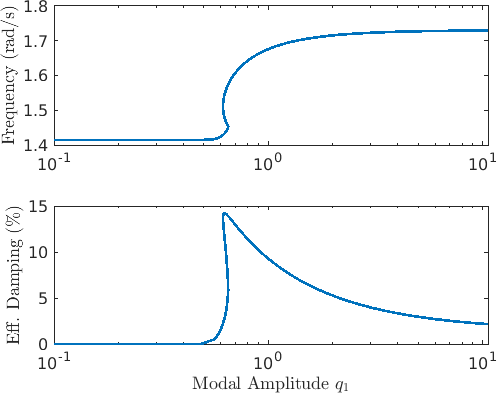
\includegraphics[width=\linewidth]{FIGS/C_EPMCBB_33_P2}
    \caption{}
  \end{subfigure}%
  \begin{subfigure}{0.5\textwidth}
    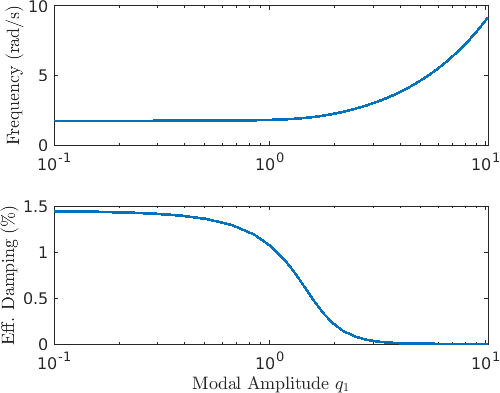
\includegraphics[width=\linewidth]{FIGS/C_EPMCBB_33_P3}
    \caption{}
  \end{subfigure}  
  \caption{Backbones for (a) friction-only ($\alpha=\gamma=0$) and (b)
    cubic spring only ($\mu N=\gamma=0$) cases (33 harmonics used for
    balance)} 
\end{figure}

The remaining parameters are identical to before.
\end{document}
%%% Local Variables:
%%% mode: latex
%%% TeX-master: t
%%% End:
